\chapter{Verification} \label{sec:design:verification}
Several of the implementation requirements have been addressed in the chapter \ref{chp:implementation}. In order to verify the implementation and there by design works, 7 tests have been conducted.
\todo{Add what has not been fully implemented}

\todo{Describe in list which requirements are tested.}
\begin{itemize}
	\item \textbf{Session Announcement (Essential metadata)}\\
This test aims to verify the Session Announcement Mechanism with Essential metadata works as intended.
	\item \textbf{Presence Mechanism}\\
This test aims to verify the Presence Mechanism works as intended.
	\item \textbf{IP collision resolver}\\
This test aims to verify the \pub{} is able to generate a new multicast IP if there is a collision.
	\item \textbf{Subscribe resolve MG}\\
This test verifies the \sub{} can tage a session name, and resolve that into an multicast IP.
	\item \textbf{Non-essential Metadata}\\
This test verifies non-essential metadata can be sent and received.
	\item \textbf{Data Integrity with \hist{}}\\
Record with tcpdump and replay with tcpreplay and see subscriber get same data.
This test verifies a stream can be recorded and replayed.
	\item \textbf{Verify RTCP SR timestamps}\\
This test is supposed to verify RTP SR timestamps are working, however at the moment of writing it does not work.
	\item \textbf{Data Integrity}\\
	Compare output from \con{} with output from \program{Snapshot}.
This verifies data sent from snapshot is the same as the \con{} receives.
\end{itemize}

\subsection{Session Announcement \& Essential Metadata} \label{sec:verify:sessionannouncement}
This test verifies implementation requirement P8,P9 and S3. The goal of the test is to verify a SDP sent by a \pub{}, and verify a \sub{} can join an announced stream. \todo{add essential metdata tot}
The test has been conducted by staring a \pub{} that streams data from a \con{} which interfaces \program{Snapshot}. In order to verify the SDP is sent as an RTP packet, the traffic sent by the \pub{} has been inspected by \program{tcpdump}. Listing \ref{cmd:verify:sdp} shows the SDP packet sent by the \pub{}.

\begin{listing}[H] 
\begin{minted}{bash}
v=0
o=suas 3736400647 3736400647 IN IP4 batbox3
s=My Session
i=A fun session
u=http://www.ecs.soton.ac.uk/fun/
t=3736400647 3736404247
a=tool:publisher.pl uuid: E9A60146-618C
m=audio 5004 RTP/AVP 96
c=IN IP6 ff15::1234/5
a=quality:5
a=rtpmap:96 L16/220500/1
\end{minted}
\caption{SDP printed by the \pub{}}
\label{lst:verify:sdp}
\end{listing}

Figure \ref{lst:verify:tcpdumpsdp} shows the output from \program{tcpdump}.

\begin{listing}[H] 
	\begin{minted}{bash}
sudo tcpdump -i eth0 -X port 5004
11:04:08.895637 IP6 batbox3.local.5004 > ff15::beef.5004: UDP, length 270
        0x0000:  6006 4601 0116 110a fe80 0000 0000 0000  `.F.............
        0x0010:  ba27 ebff fe5e 2624 ff15 0000 0000 0000  .'...^&\$........
        0x0020:  0000 0000 0000 beef 138c 138c 0116 e83d  ...............=
        0x0030:  8000 0000 0001 e240 23e2 c753 763d 300a  .......@#..Sv=0.
        0x0040:  6f3d 7375 6173 2033 3733 3634 3030 3634  o=suas.373640064
        0x0050:  3720 3337 3336 3430 3036 3437 2049 4e20  7.3736400647.IN.
        0x0060:  4950 3420 6261 7462 6f78 330a 733d 4d79  IP4.batbox3.s=My
        0x0070:  2053 6573 7369 6f6e 0a69 3d41 2066 756e  .Session.i=A.fun
        0x0080:  2073 6573 7369 6f6e 0a75 3d68 7474 703a  .session.u=http:
        0x0090:  2f2f 7777 772e 6563 732e 736f 746f 6e2e  //www.ecs.soton.
        0x00a0:  6163 2e75 6b2f 6675 6e2f 0a74 3d33 3733  ac.uk/fun/.t=373
        0x00b0:  3634 3030 3634 3720 3337 3336 3430 3432  6400647.37364042
        0x00c0:  3437 0a61 3d74 6f6f 6c3a 7075 626c 6973  47.a=tool:publis
        0x00d0:  6865 722e 706c 2075 7569 643a 2045 3941  her.pl.uuid:.E9A
        0x00e0:  3630 3134 362d 3631 3843 0a6d 3d61 7564  60146-618C.m=aud
        0x00f0:  696f 2035 3030 3420 5254 502f 4156 5020  io.5004.RTP/AVP.
        0x0100:  3936 0a63 3d49 4e20 4950 3620 6666 3135  96.c=IN.IP6.ff15
        0x0110:  3a3a 3132 3334 2f35 0a61 3d71 7561 6c69  ::1234/5.a=quali
        0x0120:  7479 3a35 0a61 3d72 7470 6d61 703a 3936  ty:5.a=rtpmap:96
        0x0130:  204c 3136 2f32 3230 3530 302f 310a       .L16/220500/1.
	\end{minted}
\caption{The listing shows the output from \program{tcpdump}, listening on the well known multicast group. The bytes shown before the SDP packet is the ethernet header, UDP header and RTP header}
\label{lst:verify:tcpdumpsdp}
\end{listing}
\todo{Insert image from wireshark where the mark bit is set.}

It should be noted that the ASCII encoded content of the payload corresponds to the SDP packet in listing \ref{lst:verify:sdp}. Furthermore, a session is announce in the key starting with \textbf{C=IN...}.

In listing \ref{lst:verify:subsdp} is the output from a \sub{} shown, that receives the SDP.


\begin{listing}[H] 
\begin{minted}{bash}
SDP from 'publisher.pl uuid: E9A60146-618C', format: audio/L16/220500/1,\
	Multicast: ff15::1234:5004
Joining multicast group: ff15::1234:5004
<SDP printet>
Main-loop stopped with retval: NewRtp
Restarting loop due to new RTP stream joined
\end{minted}
\caption{Listing shows the output from a \sub{} that receives the SDP and joins the stream. It should be noted the event-loop is restarted, in order to also listen for the new multicast group}
\label{lst:verify:subsdp}
\end{listing}

\subsection{Non-essential Metadata} \label{sec:verify:nonessentialmetadata}
This test verifies implementation requirement P7 and S6. The goal of this test is to verify non-essential metadata can be passed to a \pro{}, and read by a \con{}. 
For the test, a \textit{metadatafile.json} file created, containing the following:

\begin{listing}[H] 
\begin{minted}{json}
{
        "essential": {
        },
        "nonessential": {
          "samplerate": "100khz",
          "batbox": "batbox3",
          "number of mics: ": "2",
          "location: " : "Living room"
        }
}
\end{minted}
\caption{Listing shows example file of json encoded metadata}
\label{lst:verify:nonessentialmd}
\end{listing}

A dummy-\pro{} was written, that simply reads the file, and writes it to the metadata pipe, passed as a parameter to the \pro{}. The dummy \pro{} is shown in listing \ref{lst:verify:dummyconsumer}.

\begin{listing}[H] 
\begin{minted}{bash}
#!/bin/bash
DATA_PIPE=\$1
MD_PIPE=\$2
echo "Starting node"
cat metadata.json > \$MD_PIPE
while sleep 1; do
        echo "keepalive";
done;  
\end{minted}
\caption{Listing shows the dummy-producer implemented for testing non-essential metadata}
\label{lst:verify:dummyconsumer}
\end{listing}

\program{tcpdump} of the RTP packet has been omitted, but the payload is verified as with the SDP packet in \ref{sec:verify:sessionannouncement}.

A dummy-\con{} was written, in order to read the non-essential metadata from the pipe, and write it to a file. The dummy-\con{} and the \textit{/tmp/nonessential} is shown in listing \ref{lst:verify:dummyproducer} and \ref{lst:verify:metadataout}.


\begin{listing}[H] 
\begin{minted}{bash}
#!/bin/bash
DATA_PIPE=\$1
MD_PIPE=\$2
echo "Starting node"
if read line <\$MD_PIPE; then
	echo \$line | jq . | tee >> /tmp/nonessential
else
	echo "Running Consumer";
fi;  
\end{minted}
\caption{Listing shows the dummy-consumer reading metadata from the metadatapipe, parsing it as json, and writing it to /tmp/nonessential}
\label{lst:verify:dummyproducer}
\end{listing}



\begin{listing}[H] 
\begin{minted}{json}
{
  "number of mics: ": "2",
  "samplerate": "100khz",
  "location: ": "Living room",
  "batbox": "batbox3"
} 
\end{minted}
\caption{Listing shows the non-essential metadata from \textit{/tmp/nonessential}}
\label{lst:verify:nonessentialmetadata}
\end{listing}

\subsection{Presence Mechanism} \label{sec:verify:presencemechanism}
This test verifies implementation requirement P11-13 and S3. The goal of this test is to verify the presence mechanism works in both \sub{} and \pub{}. Due to lack of time, lists maintaining present participants have not been implemented; however, RTCP SDES/BYE are sent and received by both \pub{} and \sub{}.
A test was conducted, where the \pub{} is started and some time later the \sub{} is started. The RTCP SDES sent by the \pub{} and \sub{} is shown in figure \ref{fig:verify:wireshark_presence}.

\begin{figure}[H]
	\centering
	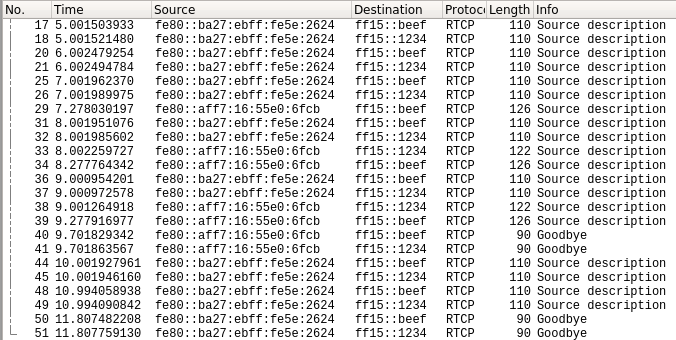
\includegraphics[width=\textwidth]{figures/wireshark_presence}
	\caption{Figure shows output from \program{Wireshark}. It should be noted, that until packet nr.26 is only fe80::ba27:.. sending RTCP SDES, but when \sub{} joins, it starts sending RTCP SDES to both the well known address ff15::beef and the source multicast group ff15::1234.} \label{fig:verify:wireshark_presence}
\end{figure}

From figure \ref{fig:verify:wireshark_presence} the RTCP SDES packets can be seen. Until packet no. 26 only the \pub{} is running. It can be seen that the \pub{} sends its RTCP SDES to both the well known multicast address(ff15::beef) and its source stream (ff15::1234). From packet nr.29, the \sub{} has been started; it sends out an RTCP SDES to the well known multicast group. It then joins the source multicast announced by the \pub{} from message no. 32, as the \sub{} sends RTCP SDES to the source stream too. From message no. 40 the \sub{} is gracefully shutting down as it sends an RTCP BYE to both source and well known multicast group. From message no. 50, the \pub{} is gracefully shutting down too.

Listing \ref{lst:verify:rtcpsdes} shows the ouput from a \sub{} receiving and parsing an RTCP SDES packet.

\begin{listing}[h] 
\begin{minted}{bash}
\$VAR1 = bless( {
                 'sdes' => {
                             '6c73c635' => {
                                             'LOC' => '',
                                             'PHONE' => '',
                                             'NAME' => '',
                                             'TOOL' => 'MCLURS',
                                             'NOTE' => '',
                                             'CNAME' => 'suas@batbox3',
                                             'EMAIL' => ''
                                           }
                           }
               }, 'Net::RTCP::Packet' );
\end{minted}
\caption{Listing shows part of the output from a \sub{} receiving and parsing an RTCP SDES packet sent by a \pub{}}
\label{lst:verify:rtcpsdes}
\end{listing}


\subsection{Data Integrity} \label{sec:verify:dataintegrity}
This test verifies that samples from \program{Snapshot} are sent and received correctly by the \con{}.
The test is conducted by running a \pub{} on a \ac{RPi}, and a \sub{} on a laptop. The laptop and the \ac{RPi} is connected over ethernet. 100 packets are sent in chunks of 4096 bytes\footnote{The default pagesize in linux}. The test is conducted by intersecting the pipe using \program{tee} between \program{Snapshot} and the \program{Publisher}, such that the samples from \program{Snapshot} can be saved to a file and sent by the \pub{}. This is depicted in figure \ref{fig:verify:dataintegrity:sketch}.

\begin{figure}[H]
	\centering
	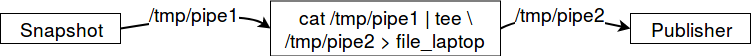
\includegraphics[width=\textwidth]{figures/dataintegrityverify.png}
	\caption{Figure shows an illustration of the intersection of the pipe between the \program{Snapshot} and the \pub{}} \label{fig:verify:dataintegrity:sketch}
\end{figure}

\noindent The \con{} has been made such that it writes all data it receives to a local file on a laptop. 
The two files are compared using \program{sha256sum}, which is sensitive to packets that have arrived out of order or not arrived at all: \\
\noindent{}Sha256sum of file from \pub{}:\\
f33c30cd3ae84e83d8bc8da7d9420d8a4639ba295eb332213132305e12b1f947 \\
\noindent{}Sha256sum of file from \sub{}:\\
f33c30cd3ae84e83d8bc8da7d9420d8a4639ba295eb332213132305e12b1f947  \\

\noindent It should be noted that both files have same sha256sum and must therefore be the same.

\subsection{Historian}
This test verifies \program{tcpdump/tcpreplay} works as \hist{}. This test has been conducted as previous test, where the data from \program{Snapshot} is saved to a file and compared to the data generated by the \con{}. This test was done by starting a \pub{} and \program{tcpdump}, in order to save the streams. The streams where then replayed using \program{tcpreplay} while a \sub{} was running. sha256 was run on the two files and compared. The result is listed below:

\noindent{}From \pub{}: \\
534b2e9f3901932eba704624281d9b8935690c9eefca1b8f0e26bc343e3d6a71\\
\noindent{}From \con{} when \program{tcpreplay} has replayed the streams\\
534b2e9f3901932eba704624281d9b8935690c9eefca1b8f0e26bc343e3d6a71\\

\noindent{}As the two hashes are the same, it shows \program{tcpdump/tcpreplay} works as a \hist{}, and that streams can be recorded and replayed.


\subsection{IP Collision Mechanism} 
This test verifies the implementation requirement P15. The goal of this test is to know if the implementation of the \pub{} is able to find a multicast group not in use by another \pub{}.
The test has been conducted by first starting one instance of \program{Publisher} and when it starts to publish data, then start a second instance of the \program{Publisher}. Both \program{Publishers} have been given the same source multicast address, namely ff15::1234.

Listing \ref{lst:verify:uniquepub1} shows the output from the first \program{Publisher}. It should be noted that it waits for 5 seconds, and then continues starting up.

\begin{listing}[H] 
\begin{minted}{bash}
Random ip: ff15::1234
Verbose: 5
Executable: producer.pl
"producer.pl" is readable
"producer.pl" is exeutable
Data pipe: /tmp/pipe_publisher_data metadata pipe:/tmp/pipe_publisher_metadata
Waitfor: duration 5.000000 and interval 1.000000
Callback invoked...
Waitfor: wake from sleep at elapsed 1.000000
Callback invoked...
Waitfor: wake from sleep at elapsed 2.000000
Callback invoked...
Waitfor: wake from sleep at elapsed 3.000000
Callback invoked...
Waitfor: wake from sleep at elapsed 4.000000
Callback invoked...
Waitfor: wake from sleep at elapsed 5.000000
Waitfor: loop completed, elapsed 5.000000 of 5.000000
No IPv6 multicast conflict
...
\end{minted}
\caption{Listing shows output from the first \pub{} running. It should be noted it does not detect a conflict, as it is the only \pub{} running}
\label{lst:verify:uniquepub1}
\end{listing}

Listing \ref{lst:implementation:uniquepub2} shows the output from the second instance of the \program{Publisher}.

\begin{listing}[H] 
\begin{minted}{bash}
Random ip: ff15::1234
Verbose: 4
Executable: producer.pl
"producer.pl" is readable
"producer.pl" is exeutable
Data pipe: /tmp/pipe_publisher_data metadata pipe:/tmp/pipe_publisher_metadata
Waitfor: duration 5.000000 and interval 1.000000
Callback invoked...
ff15::1234 vs. ff15::1234
Waitfor: loop completed, elapsed 1.000000 of 5.000000
Ipv6 multicast group conflict
New random IPv6 multicast ip: ff15::8a12
Waitfor: duration 5.000000 and interval 1.000000
Callback invoked...
ff15::1234 vs. ff15::8a12
Callback invoked...
ff15::1234 vs. ff15::8a12
Callback invoked...
ff15::1234 vs. ff15::8a12
Callback invoked...
ff15::1234 vs. ff15::8a12
Callback invoked...
ff15::1234 vs. ff15::8a12
Waitfor: loop completed, elapsed 5.000000 of 5.000000
No IPv6 multicast conflict
...
\end{minted}
\caption{Listing shows the \pub{} receives an SDP within the first second, that announces a stream on the same source multicast group as the \pub{}. }
\label{lst:verify:uniquepub2}
\end{listing}

In listing \ref{lst:verify:uniquepub2}, it receives an SDP within the first second. It continiues by generating an new source multicast group(ff15::8a12), and waits 5 seconds again to detect a conflict. At last, no conflict is discovered, and the node proceeds starting up.


\subsection{RTCP SR timeconversion}\label{sec:verify:rtcpsr}
The timeconversion does not work as intended. This has been tested by capturing 1000*2048 samples while watching the RTCP and RTP timestamps using \program{Wireshark}.  The test has been done by taking the first RTCP SR timestamp sent by the \pub{} and waiting some time and saving one more RTCP SR timestamp. By subtracting the RTP timestamps, the number of samples in the interval is known. By multiplying the number of samples by the sample period gives the time between the two RTP packets. This time should be equal to the time difference between the time in the RTCP SR timestamps, however it is not. The RTCP SR timestamp just follows the wallclock time. This could be caused by a mistake in the implementation or in the math.\\

\noindent{}The \textit{UTC offset} estimation is known to work, as it has been tested as shown in figure \ref{lst:verify:utcoffset}. The test has been conducted by calculating the time from the \program{Snapshot} by adding its monotonic clock to the offset before and after the program has slept for 5 seconds. After the 5 seconds, there is 5 seconds between the timestamps estimated from the monotonic clock and from the realclock.  Both of these datetimes are in UTC.

\begin{listing}[H] 
\begin{minted}{bash}
Calculating offset
Offset: 1527354387.73806
Datetime from Ztatus: 2018-05-27T22:11:36 realclock: 2018-05-27T22:11:36
Sleeping 5 seconds
Datetime from Ztatus: 2018-05-27T22:11:41 realclock: 2018-05-27T22:11:41
localtime: Mon May 28 00:11:41 2018
\end{minted}
\caption{Listing shows the output of test script to calculate time offset between the realtime and random monotonic clock from \textit{Snapshot}}
\label{lst:verify:utcoffset}
\end{listing}

It should be noted from listing \ref{lst:verify:utcoffset} that there is 2 hours offset from the localtime to the timestamps of the estimated UTC offset.  This is due to the timezone in Denmark at the moment of writing is GMT+2.

\noindent{}By inspection of packets in \program{Wireshark}, it can be seen the RTP timestamp is incremented 2048 for each packet as expected.


